\documentclass[11pt]{article}
\usepackage{lmodern}
\usepackage[T1]{fontenc}
\usepackage[latin9]{inputenc}
\usepackage{geometry}
\geometry{verbose,tmargin=2.54cm,bmargin=2.54cm,lmargin=2.54cm,rmargin=2.54cm}
\usepackage{color}
\usepackage{verbatim}
\usepackage{float}
\usepackage{amsmath}
\usepackage{graphicx}
\usepackage{setspace}
\usepackage[authoryear]{natbib}
\onehalfspacing
\usepackage[unicode=true,pdfusetitle,
bookmarks=true,bookmarksnumbered=false,bookmarksopen=false,
breaklinks=false,pdfborder={0 0 1},backref=false,colorlinks=true]
{hyperref}
\hypersetup{
	citecolor=blue, urlcolor = brown }
%\usepackage{breakurl}
\usepackage{caption}
\usepackage{pdflscape}
\usepackage{multirow} %http://ctan.org/pkg/multirow
\usepackage{longtable}
\makeatletter
\usepackage{endnotes}
\usepackage{longtable}
\usepackage{lscape}
\usepackage{array}
\usepackage{adjustbox}
\usepackage{tabularx}
\usepackage{threeparttable}
\setcitestyle{citesep={;}, aysep={,}}
\usepackage{booktabs}% Allows the use of \toprule, \midrule and \bottomrule in tables for horizontal lines
\usepackage{float}
\usepackage{subcaption}
\definecolor{green}{RGB}{0, 180, 0}
\definecolor{blue}{RGB}{0,46,180}
\definecolor{brown}{RGB}{165,42,42}

\usepackage{colortbl}
\usepackage{ragged2e}
\usepackage{xfp}
% To allow textsubscript in section titles:

\usepackage{stackengine}
\usepackage{array}
\newcolumntype{L}[1]{>{\raggedright\arraybackslash}p{#1}}
\setstackEOL{\#}
\setstackgap{L}{12pt}




\title{\underline{Preliminary results} \linebreak
	Cross-grade ability grouping in Liberia}
\date{\today}

\makeatother

\begin{document}
	\maketitle

\centering

\section*{Main results }

\begin{table}[H]
	\begin{center} 
\caption{\small Effects on test scores} 
\label{tab:descriptives} 
\begin{small}
\begin{threeparttable}
\begin{tabular} {@{} l l c c c c @{}} \toprule \toprule
&&\Longstack{Control\#mean}&\Longstack{Coef.}&\Longstack{N}  \\
&&(1)&(2)&(3) \\ \midrule 
\\
&Stacked &0.092&-0.246*&3,147 \\
&                &&(0.140)&  \\
&Grades 3-4 &0.060&-0.396**&1,470 \\
&                &&(0.190)&  \\
&Grades 1-2 &0.119&-0.097&1,677 \\
&                &&(0.196)&  \\
\midrule
\bottomrule
\end{tabular}
\begin{tablenotes}
\item Notes: All specifications control linearly for randomization strata fixed effects and predicted ability. Standard errors are clustered at the academy-grade group level. ***, **, and * indicate significance at 1\%, 5\%, and 10\%. \end{tablenotes}
\end{threeparttable}
\end{small}
\end{center}
\clearpage

\end{table}

\begin{table}[H]
	\begin{center} 
\caption{\small The Effect of treatment by upper or lower group placement} 
\label{tab:descriptives} 
\begin{small}
\begin{threeparttable}
\begin{tabular} {@{} l l c c c   @{}} \toprule \toprule
& Stacked & Grades 3-4 & Grades 1-2 & \\
 \\ \midrule 
\\
 Treatment      &  -0.03  &  -0.03  &  -0.02   \\
             &  (0.18)  &  (0.30)  &  (0.20)   \\
 Treatment $\times$ Upper group      &  -0.37*  &  -0.42  &  -0.14   \\
             &  (0.21)  &  (0.32)  &  (0.25)   \\
 Upper group      &  0.41***  &  0.43*  &  0.44**   \\
             &  (0.15)  &  (0.24)  &  (0.19)   \\
\midrule
Pval: Treatment + Treatment $\times$ Upper group     &  0.02  &  0.03  &  0.53   \\
Observations     & 3,147  & 1,470  & 1,677   \\
\bottomrule
\end{tabular}
\begin{tablenotes}
\item Notes: All specifications control linearly for randomization strata fixed effects. Standard errors are clustered at the academy-grade group level. ***, **, and * indicate significance at 1\%, 5\%, and 10\%. \end{tablenotes}
\end{threeparttable}
\end{small}
\end{center}
\clearpage

\end{table}


\begin{table}[H]
	\begin{center} 
\caption{\small Effect on within-class dispersion in test scores} 
\label{tab:descriptives} 
\begin{scriptsize}
\begin{threeparttable}
\begin{tabular} {@{} l l c c c c c c c c @{}} \toprule \toprule
&& \multicolumn{3}{c}{Predicted ability} &&  \multicolumn{3}{c}{Actual outcomes}
&&\multicolumn{3}{c}{}&&\multicolumn{3}{c}{} \\  \cmidrule{3-5} \cmidrule{7-9} 
&&\Longstack{Control\#mean}&\Longstack{Coef.}&\Longstack{N}&&\Longstack{Control\#mean}&\Longstack{Coef.}&\Longstack{N}  \\
&&(1)&(2)&(3)&&(4)&(5)&(6) \\ \midrule 
\\
&Stacked & 0.546&0.072&4,774&& 0.459&0.101**&3,147 \\
&                && (0.046)&&&& (0.047)& \\
&Grades 3-4 & 0.584&0.030&2,361&& 0.488&0.136***&1,470 \\
&                && (0.068)&&&& (0.054)& \\
&Grades 1-2 & 0.509&0.106**&2,413&& 0.436&0.054&1,677 \\
&                && (0.054)&&&& (0.071)& \\
\midrule
\bottomrule
\end{tabular}
\begin{tablenotes}
\item Notes: The outcome is the absolute deviation of each student's standardized test score from the classroom mean. All specifications control linearly for randomization strata fixed effects. Standard errors are clustered at the academy-grade group level. ***, **, and * indicate significance at 1\%, 5\%, and 10\%.\end{tablenotes}
\end{threeparttable}
\end{scriptsize}
\end{center}
\clearpage

\end{table}

\begin{table}[H]
	\begin{center} 
\caption{\small Effect on test scores} 
\label{tab:descriptives} 
\begin{small}
\begin{threeparttable}
\begin{tabular} {@{} l l  c c c  @{}} \toprule \toprule
 & & Stacked & Grades 3-4  & Grades 1-2 \\
& &(1)&(2)&(3) \\ \midrule 
\\
Mean peer ability &  & 0.013* & 0.020** & 0.003 \\
                 &  & (0.007) & (0.009) & (0.012) \\
Distance from median instruction &  & -0.056** & -0.102** & -0.006 \\
                 &  & (0.028) & (0.044) & (0.026) \\
Class size &  & 0.003 & 0.002 & 0.008 \\
                 &  & (0.005) & (0.005) & (0.009) \\
\midrule
Number of students &  & 3147 & 1470 & 1677 \\
Number of schools &  & 54 & 54 & 54 \\
\bottomrule
\end{tabular}
\begin{tablenotes}
\item Notes: All specifications control linearly for randomization strata fixed effects and predicted ability. Each specification also controls for the expected value of the respective independent variable used in the specification. Standard errors are clustered at the academy-grade group level. ***, **, and * indicate significance at 1\%, 5\%, and 10\%.\end{tablenotes}
\end{threeparttable}
\end{small}
\end{center}
\clearpage

\end{table}

\begin{figure}[ht!]
        \centering
       \caption{Distribution of Baseline Test Scores}        
        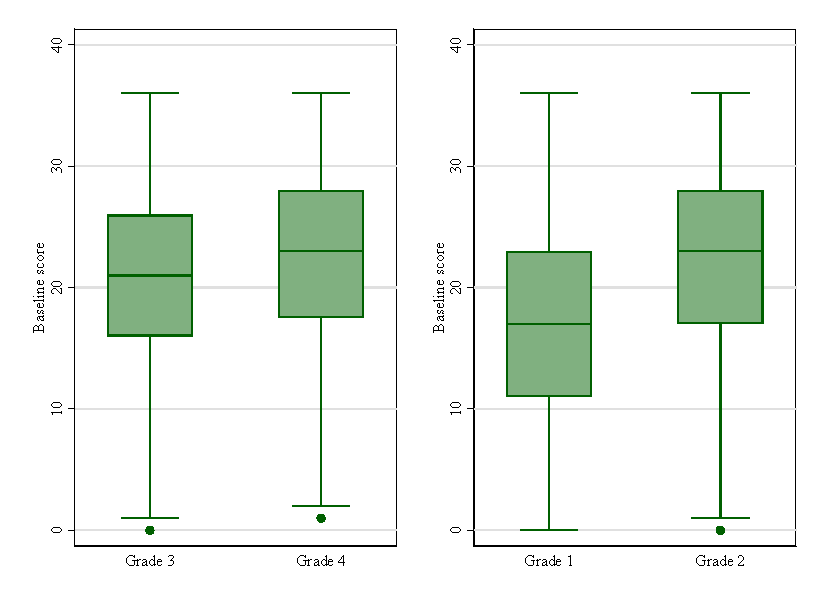
\includegraphics[width = 5in]{Liberia2024/bxplt_lib.pdf}
\end{figure}

\begin{figure}[ht!]
        \centering
       \caption{Endline achievement by predicted ability deciles (Grades 3-4)}        
        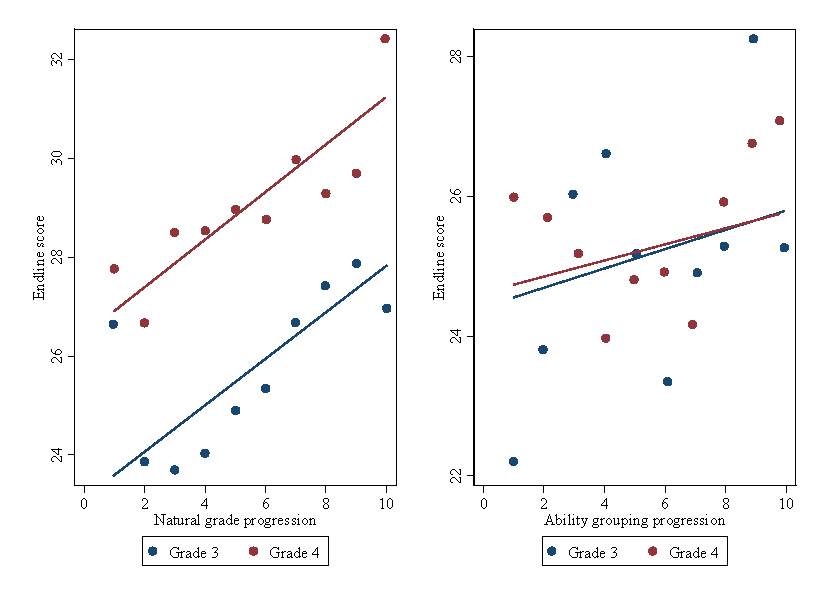
\includegraphics[width = 5in]{Liberia2024/q_34_lib.pdf}
\end{figure}

\begin{figure}[ht!]
        \centering
       \caption{Endline achievement by predicted ability deciles (Grades 1-2)}        
        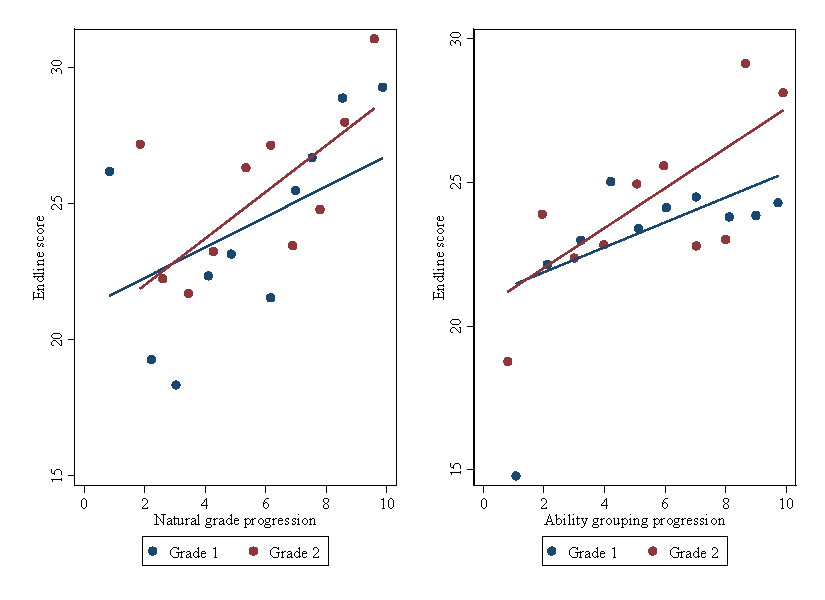
\includegraphics[width = 5in]{Liberia2024/q_12_lib.pdf}
\end{figure}

\begin{figure}[ht!]
        \centering
       \caption{Distribution of predicted ability (Grades 3-4)}        
        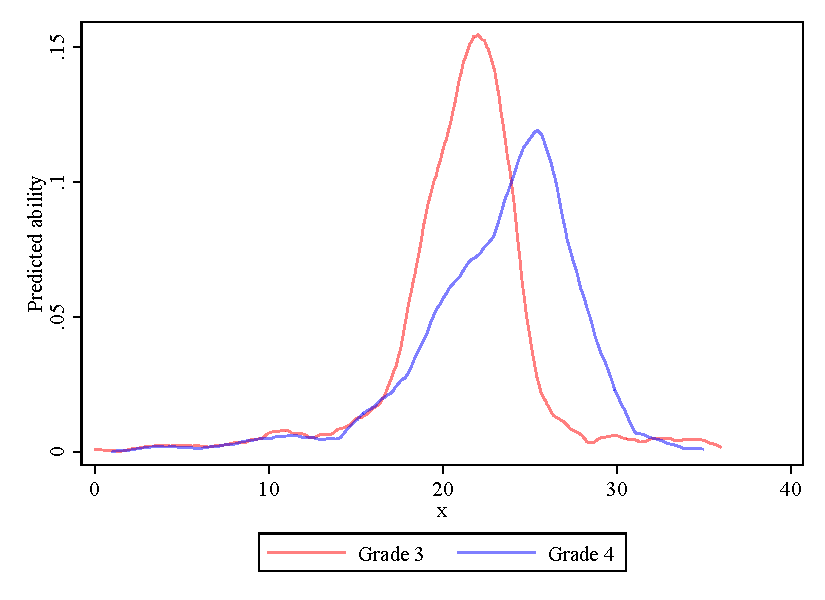
\includegraphics[width = 5in]{Liberia2024/ability_dist34_lib.pdf}
\end{figure}

\begin{figure}[ht!]
        \centering
       \caption{Distribution of predicted ability (Grades 1-2)}        
        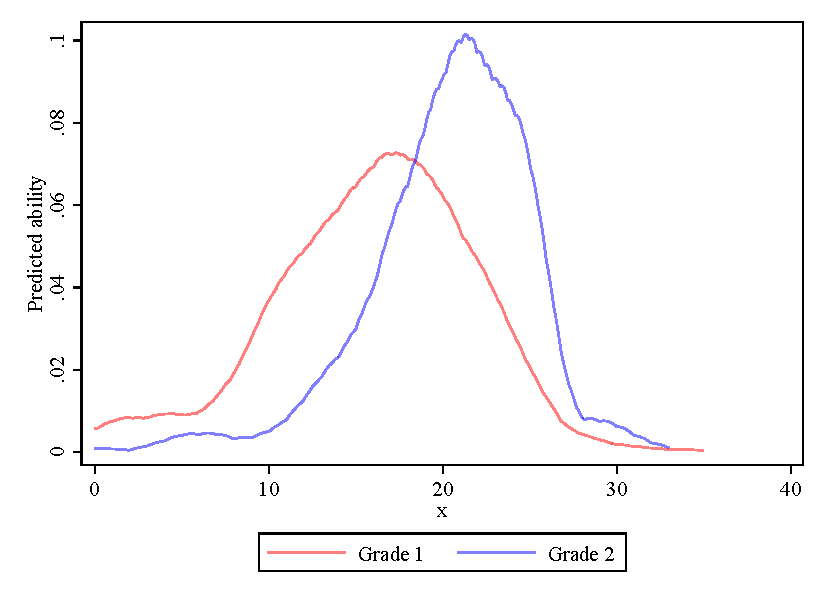
\includegraphics[width = 5in]{Liberia2024/ability_dist12_lib.pdf}
\end{figure}

\begin{figure}[ht!]
        \centering
       \caption{Predicted ability (Empirical Bayes) vs. test scores}      
        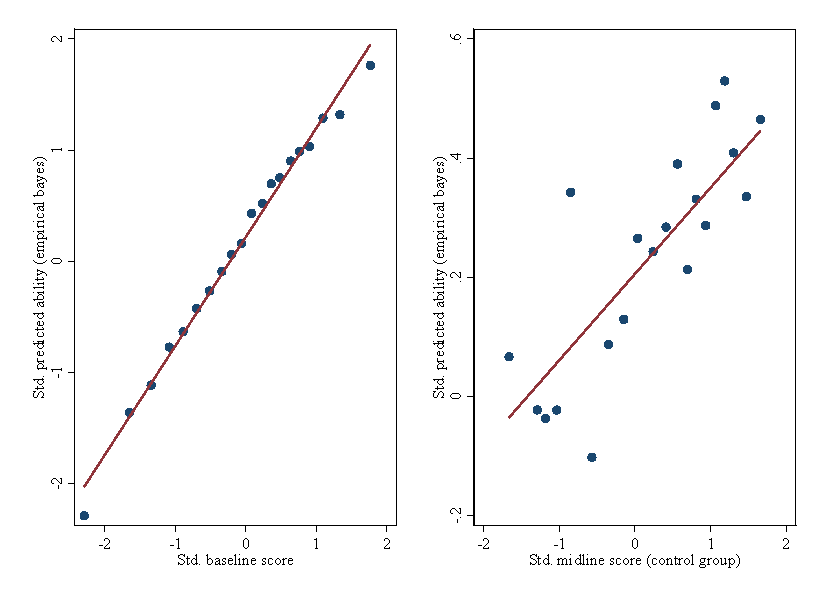
\includegraphics[width = 5in]{Liberia2024/corr_bl_eb.pdf}
        \caption*{Notes: The predicted ability scores were estimated using an empirical bayes procedure. This procedure combined individual-level baseline scores and (control) group-level midline scores. Shrinkage weights were calculated based on the inverse variance of the baseline and control group midline test scores, assigning higher weight to the more reliable (lower variance) measure. For cases where midline scores were missing, individual baseline scores were used as a fallback.}
\end{figure}



\end{document}  